% !TeX root = ../thuthesis-caishiyu.tex

\chapter{实验与评价}

本章节主要介绍 N2DB 的垃圾回收机制以及数据恢复机制的实验与评价。
本文使用 TPC-C 以及 YCSB 两种实验负载对 N2DB 以及 InnoDB 进行实验,主要的测试目标为:
\begin{itemize}
    \item N2DB 在开启和关闭垃圾回收机制下系统的运行性能对比以及存储空间使用量对比
    \item N2DB 和 MySQL 在相同条件下数据恢复的时间对比以及存储空间使用量对比
\end{itemize}

本章节首先介绍实验的环境设置,包括实验环境的硬件条件,NVM 的工作模式以及两个系统的参数设置。接着本章节介绍使用的两个负载的基本情况以及参数设置。之后的章节将会从垃圾回收以及数据恢复两个方面进行实验,并对实验数据进行分析。

\section{实验设置}

本文的实验均在同一台服务器上运行。该服务器有 4 个 Intel Xeon Gold 5220 处理器。每个处理器上有 18 个核。
Intel Optane DC PMM 是安装在处理器的内存插槽的。一个处理器有 6 个内存插槽,Intel Optane DC PMM 的容量是 128 GB,因此一个处理器的 NVM 空间至多为 768 GB。由于非统一内存访问(NUMA)效应,线程跨核访问 NVM 空间的性能会显著下降。因此本文的实验均在同一个核上进行。本实验中 NVM 的使用模式有 DAX 模式以及文件系统模式,两种模式的性能差异如表格~\ref{tab:nvm-metric} 所示。

\begin{table}
    \centering
    \caption{NVM 文件系统模式以及 DAX 的模式的访问性能对比}
    \begin{tabular}{lll}
        \toprule
        指标           & 文件系统模式 & DAX 模式 \\
        \midrule
        读带宽(GB/s) & 4.7          & 23       \\
        写带宽(GB/s) & 1.8          & 11       \\
        读延迟(ns)   & 1700         & 310      \\
        写延迟(ns)   & 5500         & 105      \\
        \bottomrule
    \end{tabular}
    \label{tab:nvm-metric}
\end{table}

本文用于对比的系统是 InnoDB。InnoDB 是 MySQL 的存储引擎,其接口与 N2DB 十分相近。
在本实验中,InnoDB 使用文件系统模式使用 NVM 空间。
InnoDB 使用 WAL 来记录事务的操作,同时使用 ARIES 算法来进行数据恢复。
$log\_file\_size$ 是 InnoDB 的一个影响恢复性能的重要参数,其含义为 InnoDB 的日志文件大小。
通常 InnoDB 的日志数量为两个,InnoDB 会交替使用两个日志。当一个日志写满时,InnoDB 会进行一次 checkpoint 操作,之后切换到另外一个日志。因此 $log\_file\_size$ 影响 InnoDB 的运行时性能以及恢复时的性能。当 $log\_file\_size$ 越大时,InnoDB 生产 checkpoint 的频率越低,系统运行时的性能提高。但是 checkpoint 的频率降低意味着 InnoDB 在重启之后需要处理的日志的数量增多,因此会增加恢复时间,同时也会增大存储空间的使用量。在本文中,$log\_file\_size$ 被设置为 64 MB,128 MB 以及 256 MB。
InnoDB 使用文件系统模式访问和管理 NVM。

N2DB 在本实验中使用 $gc\_threshold$ 参数来控制垃圾回收的频率。在垃圾回收的对比实验中,gc\_threshold 被设置为 100。

\section{实验负载}

本实验使用 YCSB 以及 TPC-C 两种实验负载来测试 N2DB 的垃圾回收机制和数据恢复机制的性能。

YCSB 是雅虎公司对云服务进行性能测试的工具。YCSB 主要测试的事务操作是读,更新以及范围查询。
YCSB 的测试数据库中仅有一个张表格。表格中一共有 10 列,其中包含一个主键以及 9 个字节类型的列。每列的长度为 10 字节,因此一条记录为 100 字节。本实验中 YCSB 的测试表格中一共有 1000000 条记录。表格的数据大小在 1 GB 左右。
YCSB 中的每个事务会进行 10 次操作,每次操作的类型是随机的。本实验中所使用 YCSB 根据操作类型的分布可以分为三类,分别是:
\begin{enumerate}
    \item \textbf{读偏向型:}$90\%$ 读操作,$10\%$ 写操作;
    \item \textbf{平衡型:}$50\%$ 读操作,$50\%$ 写操作;
    \item \textbf{写偏向型:}$10\%$ 读操作,$90\%$ 写操作;
\end{enumerate}


TPC-C 是针对联机交易类型(OLTP)数据库设计的性能测试工具。TPC-C 模拟了一个电商环境。在该环境中,用户可以发布新的交易订单,供应商会根据仓库以及辖区的存储信息进行货物配送以及资金结算。
TPC-C 的测试数据库一共包含 9 张表,包括仓库,用户,订单等。TPC-C 测试中,事务会按照一定分布执行 5 个类型的操作。在本文的实验设置中,仓库数量固定为 8 个,并且所有表格数据初始大小控制在 1 GB 左右。

\section{垃圾回收性能对比实验}

本章节将比较开启与关闭垃圾回收机制对于系统运行时性能以及存储空间的影响。本章节将使用三种类型的 YCSB 以及 TPC-C 进行实验。

\begin{figure}
    \centering
    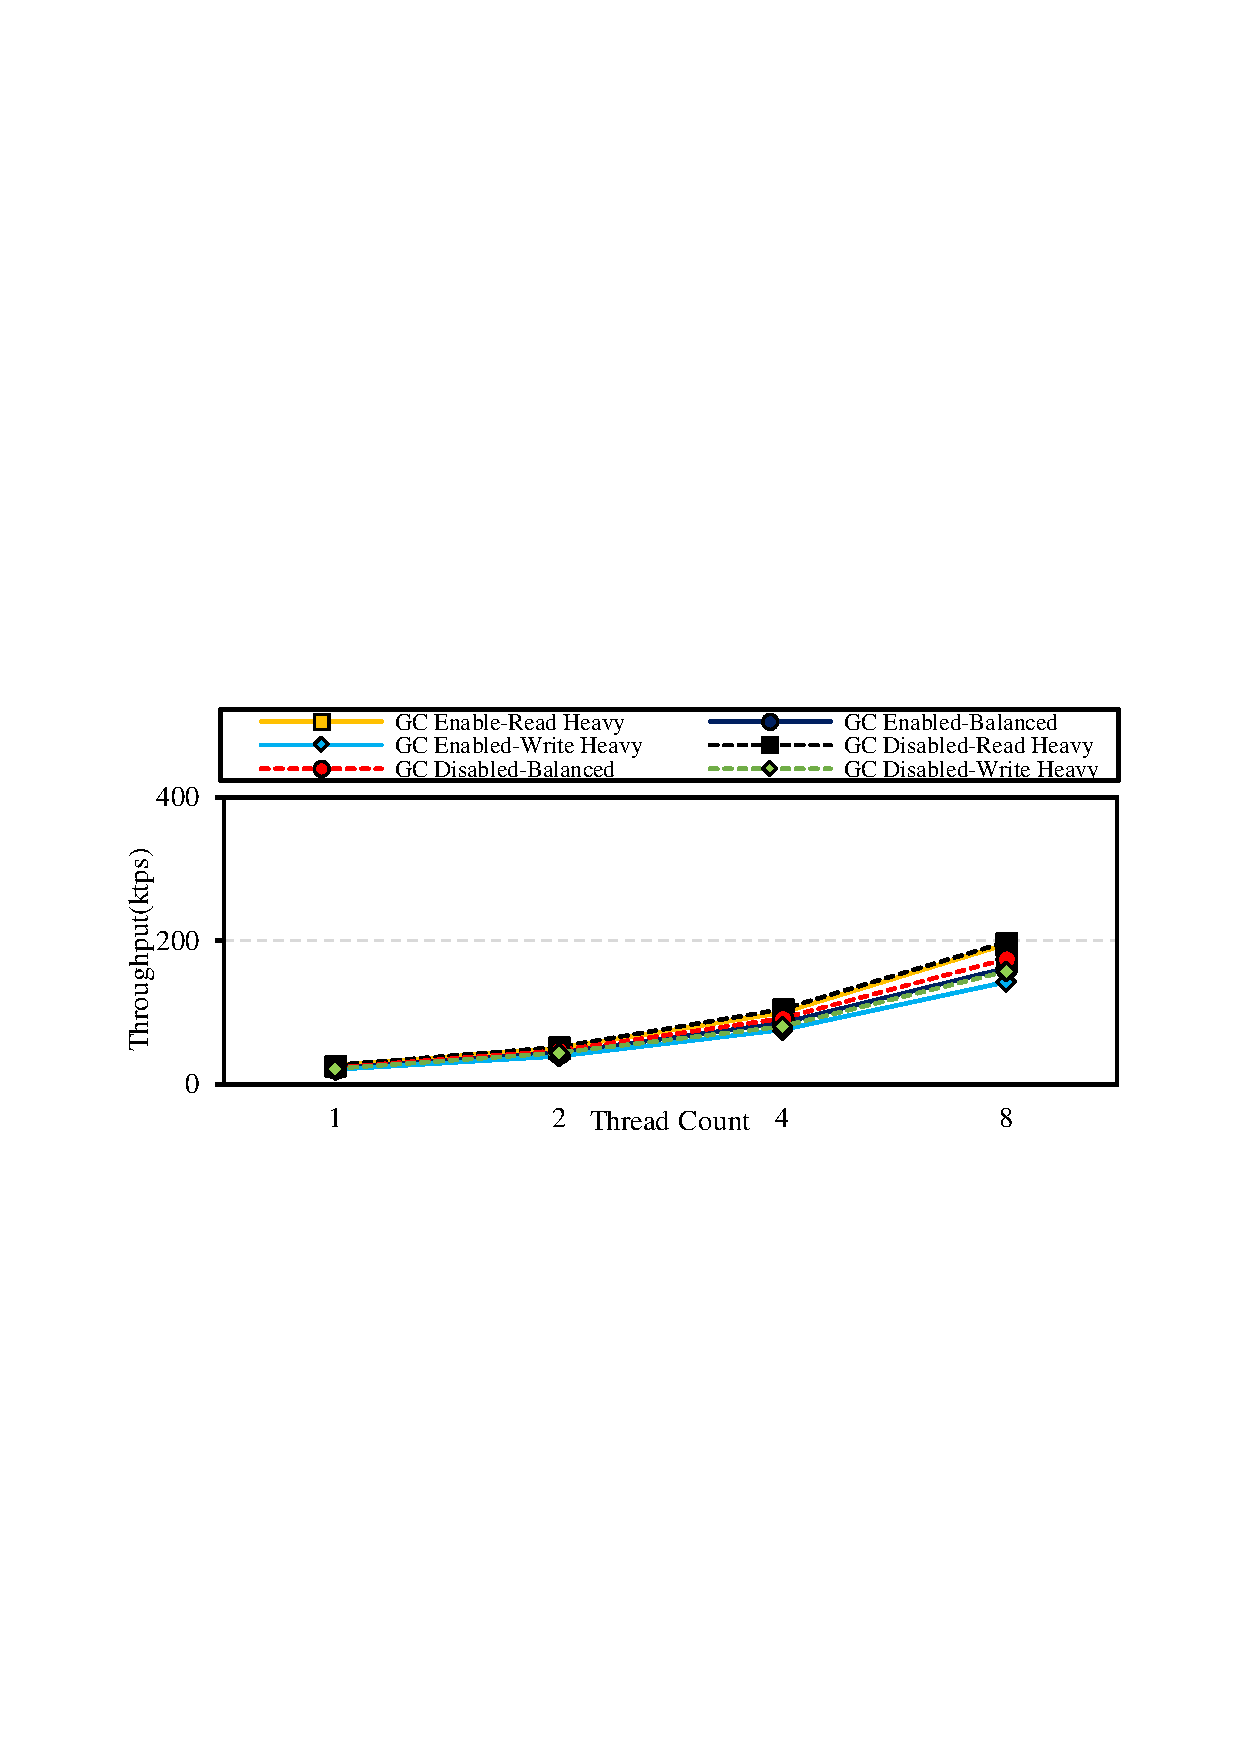
\includegraphics[width=15cm, trim={1cm 9cm 1cm 10cm}]{figures/gc-ycsb-throughput.pdf}
    \caption{YCSB 负载下垃圾回收性能的吞吐率对比实验}
    \label{fig:gc-throughput-ycsb}
\end{figure}

\subsection{运行时性能对比}

首先是三种 YCSB 负载下的运行时性能对比。如图~\ref{fig:gc-throughput-ycsb} 所示,整体上开启垃圾回收比关闭垃圾回收的运行时性能至多慢 $10\%$。在读偏向型的 YCSB 负载下,开启垃圾回收的系统性能比关闭垃圾回收的系统少 $2\%$ 左右。这是因为读偏向型负载下,事务更新数量少,因此产生的不可见版本少,没有垃圾回收的必要,而且垃圾回收机制本身引入了额外的开销。平衡型的实验结果也与读偏向型负载相似,开启垃圾回收的系统的吞吐率相对于关闭的系统少约 $7\%$。写偏向型的实验结果中,单核时开启的系统相对于关闭的系统少 $7\%$。随着核数增多,这个差异增大到 $10\%$。这是因为引入垃圾回收会增大线程之间冲突的概率,额外的锁开销也会影响运行时的事务的性能。因此二者的差异会随着核数的增加而增加。


\begin{figure}
    \centering
    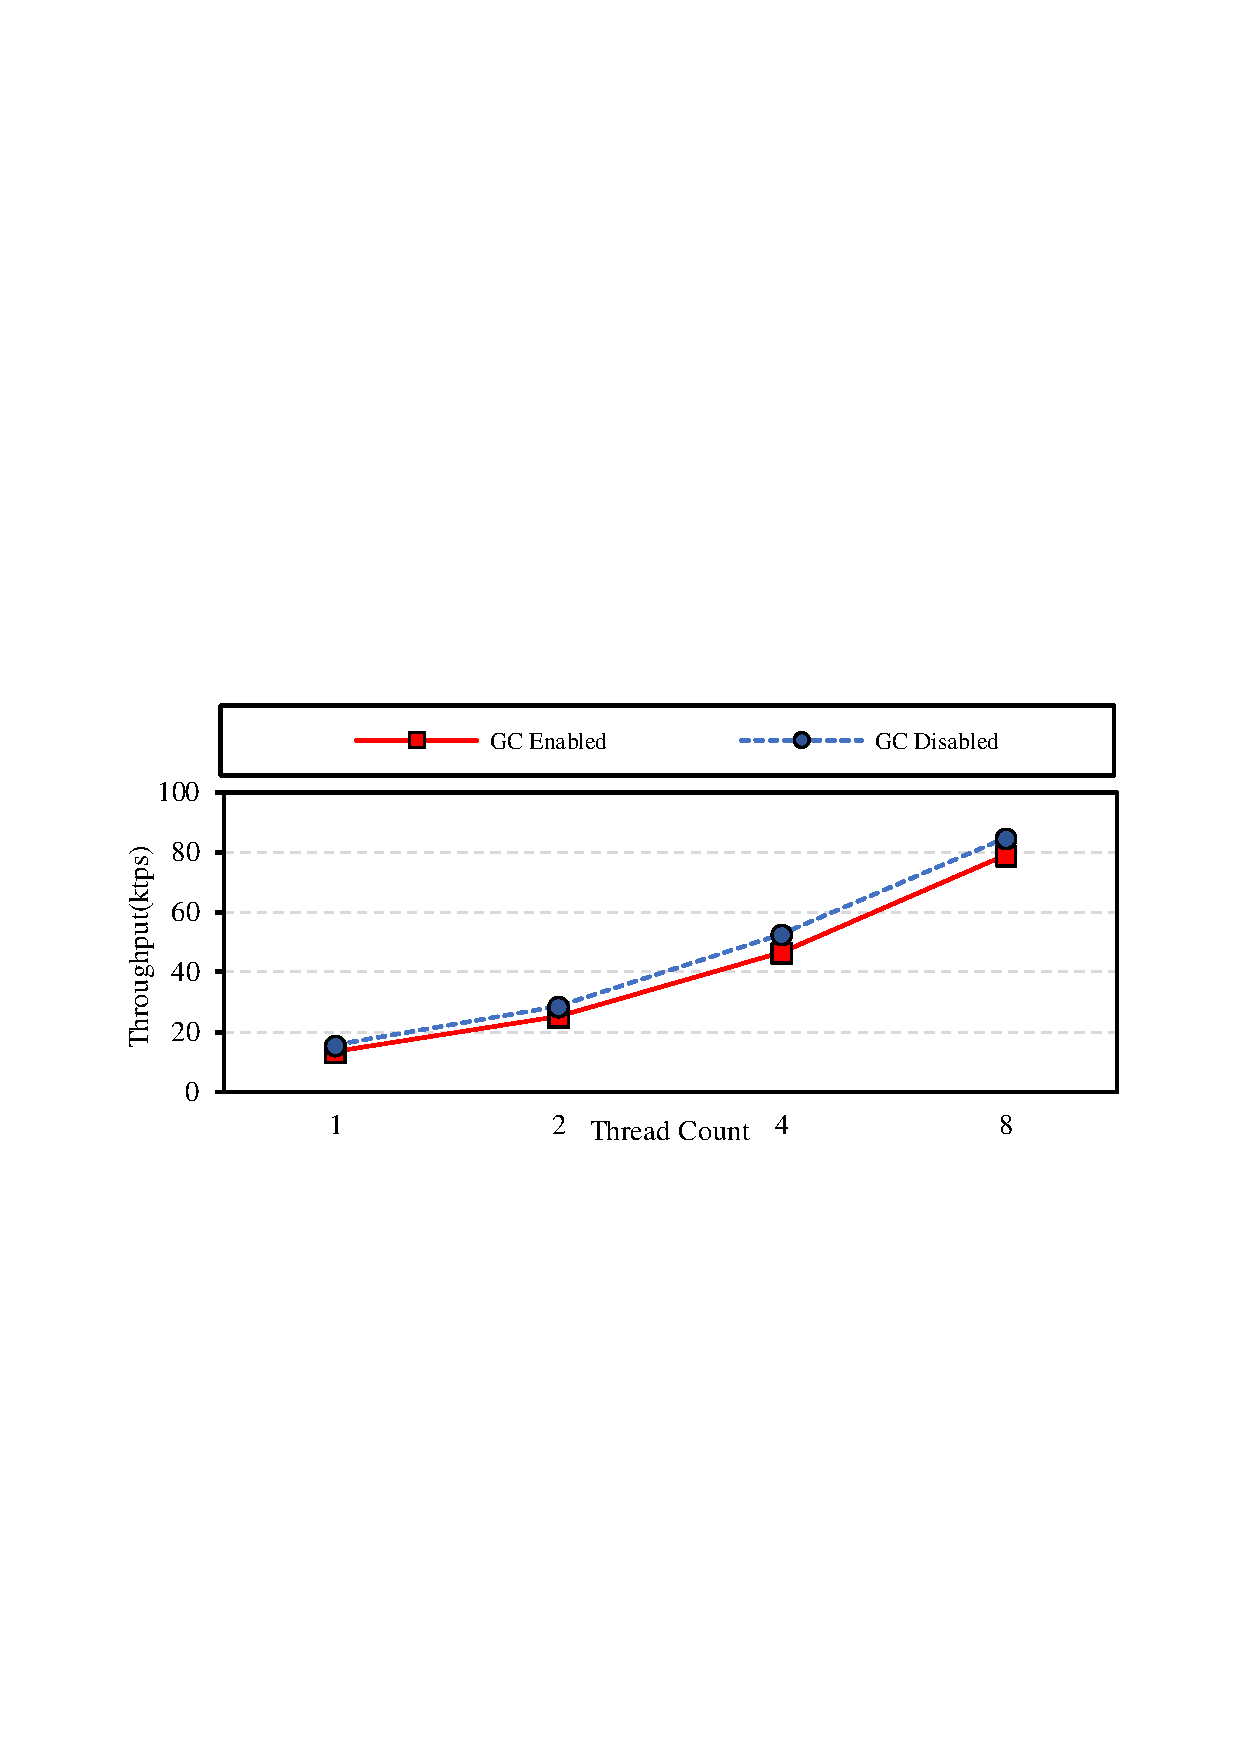
\includegraphics[width=15cm, trim={1cm 9cm 1cm 10cm}]{figures/gc-tpcc-throughput.pdf}
    \caption{TPC-C 负载下垃圾回收性能的吞吐率对比实验}
    \label{fig:gc-throughput-tpcc}
\end{figure}

接下来是 TPC-C 负载下的运行时性能对比。如图~\ref{fig:gc-throughput-tpcc} 所示,TPC-C 负载下的性能差异与写偏向型的 YCSB 负载下的性能差异相近。这是因为 TPC-C 负载中,事务的操作类型大多是更新操作。



\subsection{存储空间对比}

三种 YCSB 以及 TPC-C 负载下的存储空间对比如图~\ref{fig:gc-storage-ycsb} 以及图~\ref{fig:gc-storage-tpcc} 所示。
在读偏向型的 YCSB 负载的实验结果中,开启垃圾机制至多节省 $20\%$ 左右的存储空间。
随着负载中的更新事务的占比的提高,垃圾回收所节省的存储空间的比例也逐渐上升。
平衡型 YCSB 负载中垃圾回收至多节约了 $55\%$,而在写偏向型负载和 TPC-C 负载中,对应的比例分别为 $67\%$ 和 $50\%$。

\begin{figure}
    \centering
    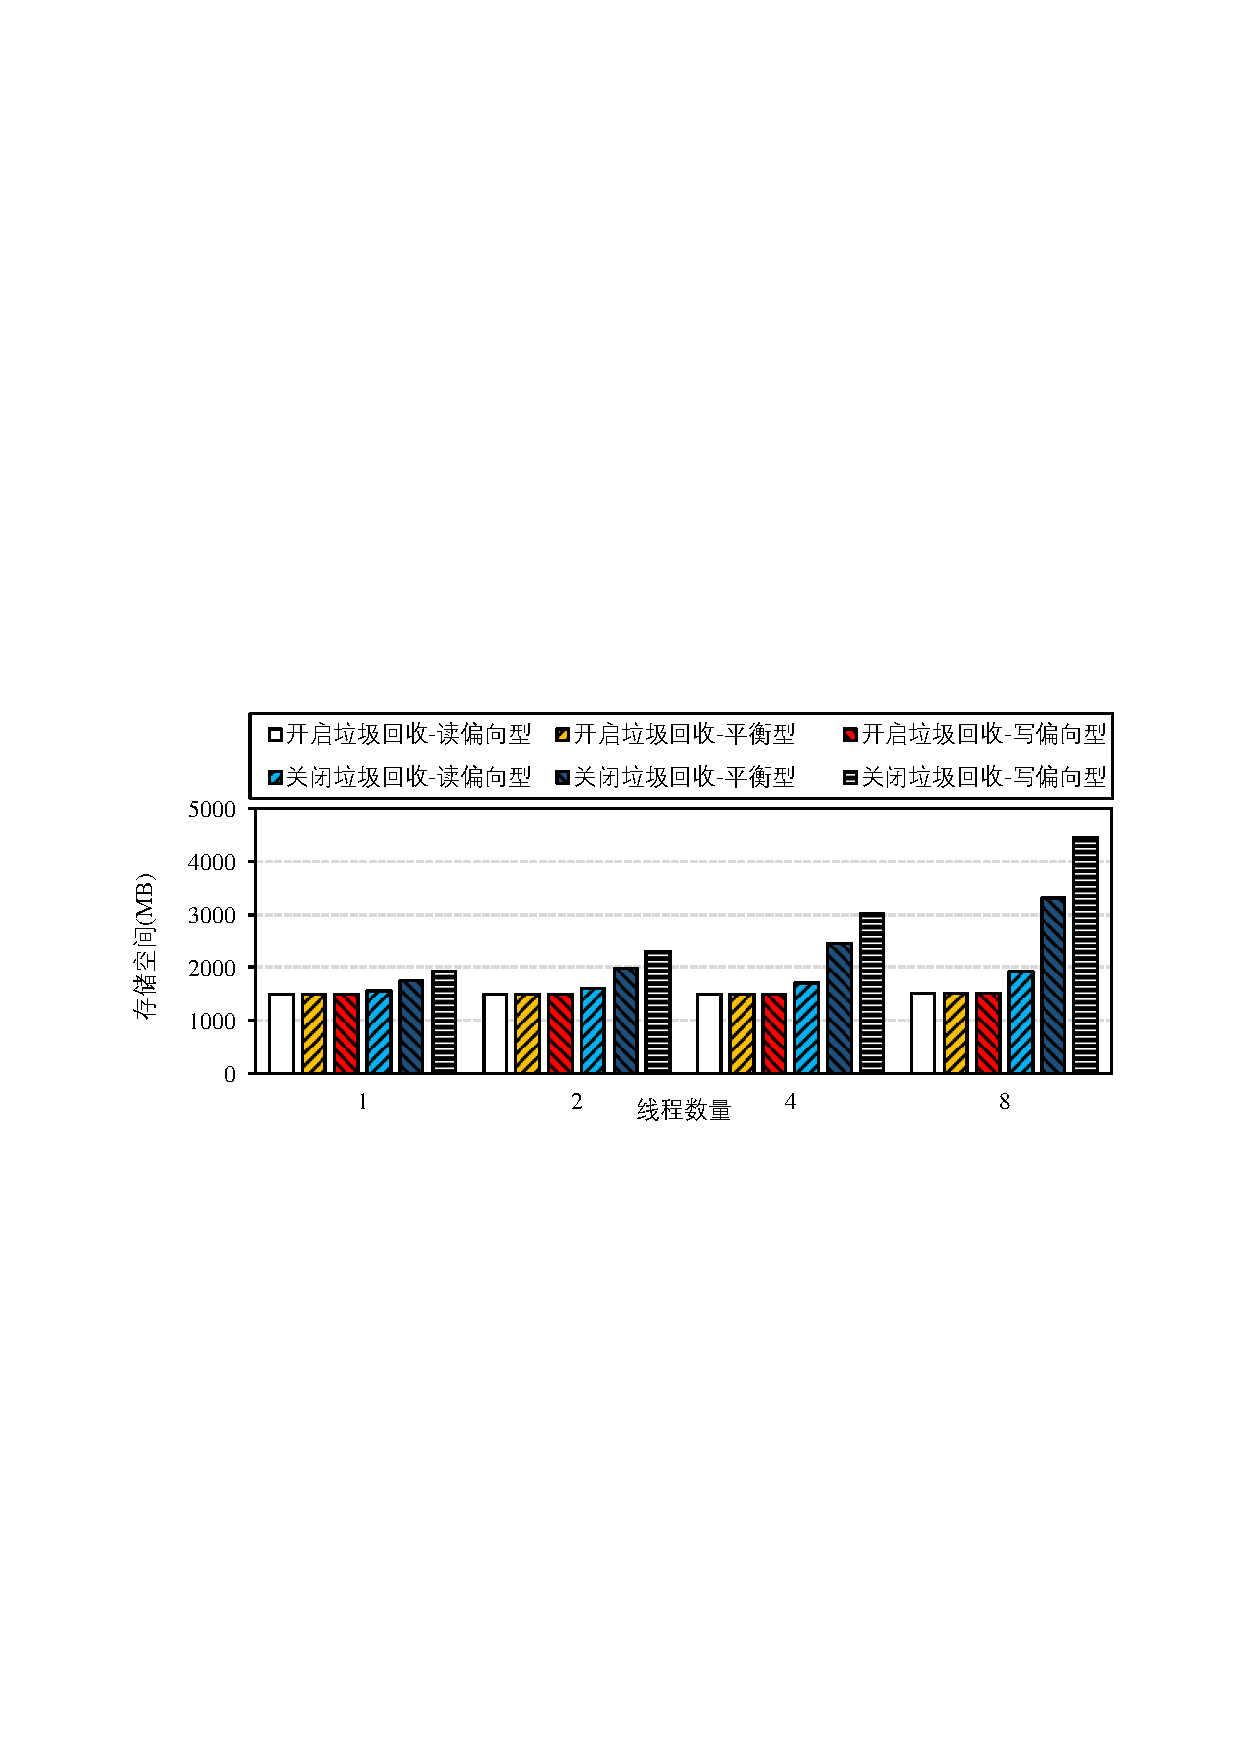
\includegraphics[width=15cm, trim={1cm 9cm 1cm 10cm}]{figures/gc-ycsb-storage.pdf}
    \caption{YCSB 负载下垃圾回收性能的存储空间对比实验}
    \label{fig:gc-storage-ycsb}
\end{figure}

\begin{figure}
    \centering
    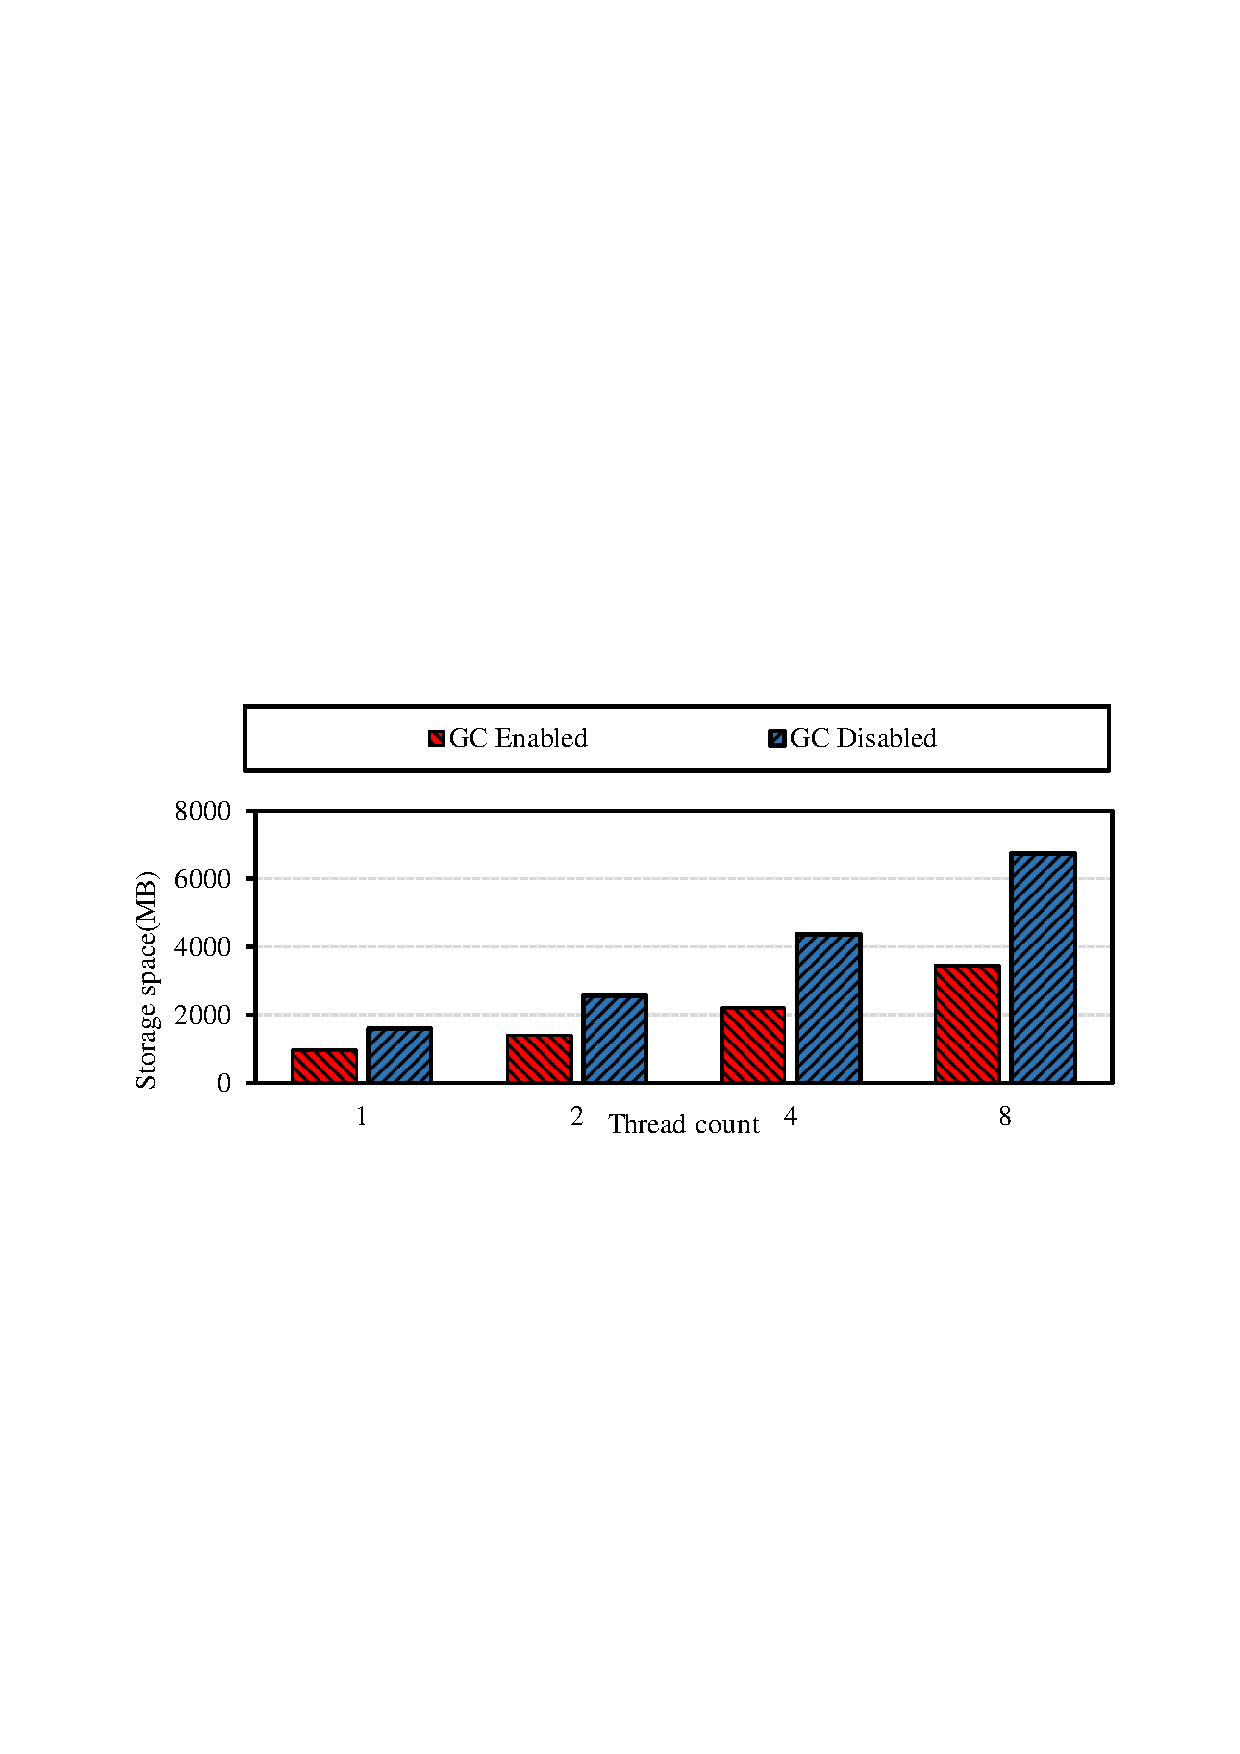
\includegraphics[width=15cm, trim={1cm 9cm 1cm 10cm}]{figures/gc-tpcc-storage.pdf}
    \caption{TPC-C 负载下垃圾回收性能的存储空间对比实验}
    \label{fig:gc-storage-tpcc}
\end{figure}

整体上而言,垃圾回收机制对于 N2DB 此类基于多版本并发控制的算法的系统效果显著。
并且效果随着系统中的更新操作的所占的比重增加而增加。


\section{数据恢复性能对比实验}

本章节将对比 N2DB 与 InnoDB 的数据恢复性能。两个系统均使用平衡型的 YCSB 负载。
当事务提交的数量达到一个阈值时,测试工具将使用 SIGKILL 强制结束两个系统,之后记录两个系统的恢复时间以及存储空间使用情况。在本实验中,实验使用不同提交事务的阈值来进一步对比恢复性能差异。在本实验设置中,提交事务的阈值分别是 10000 和 100000。

\subsection{数据恢复时间对比}

首先是在数据恢复的时间对比。实验结果如图~\ref{fig:recovery-time-ycsb} 所示。
总体上而言,N2DB 的恢复时间远小于 InnoDB 的恢复时间。前者大约比后者小三个数量级。
造成这一差异的主要原因在于基于 WAL 的恢复机制的复杂性。
该机制要求系统在数据恢复时扫描日志,分析系统中断的状态。
之后系统需要重做检查之后的所有日志来将系统的状态恢复到系统故障的时刻的状态。
最后在回滚阶段,系统需要回滚所有未提交事务的操作。
并且该机制要求系统只有在回滚操作全部结束后才能相应服务。
N2DB 从并发控制算法的角度保证了提交事务的影响的持久化,因此在数据恢复时不需要重做。
对于 N2DB 中的中止事务的影响,对于 head 的影响会被立刻回收,而对于 version 的影响会根据可见性判断无视掉。
N2DB 仅需要得到索引重建之后就能提供服务。

从 InnoDB 的实验结果可以看出,不同的 $log\_file\_size$ 会显著影响恢复时间。
在本文的实验中,256 MB 相对于 64 MB 仅能带来 $10\%$ 的性能提升,同时会导致恢复时间提高 $70\%$。


\begin{figure}
    \centering
    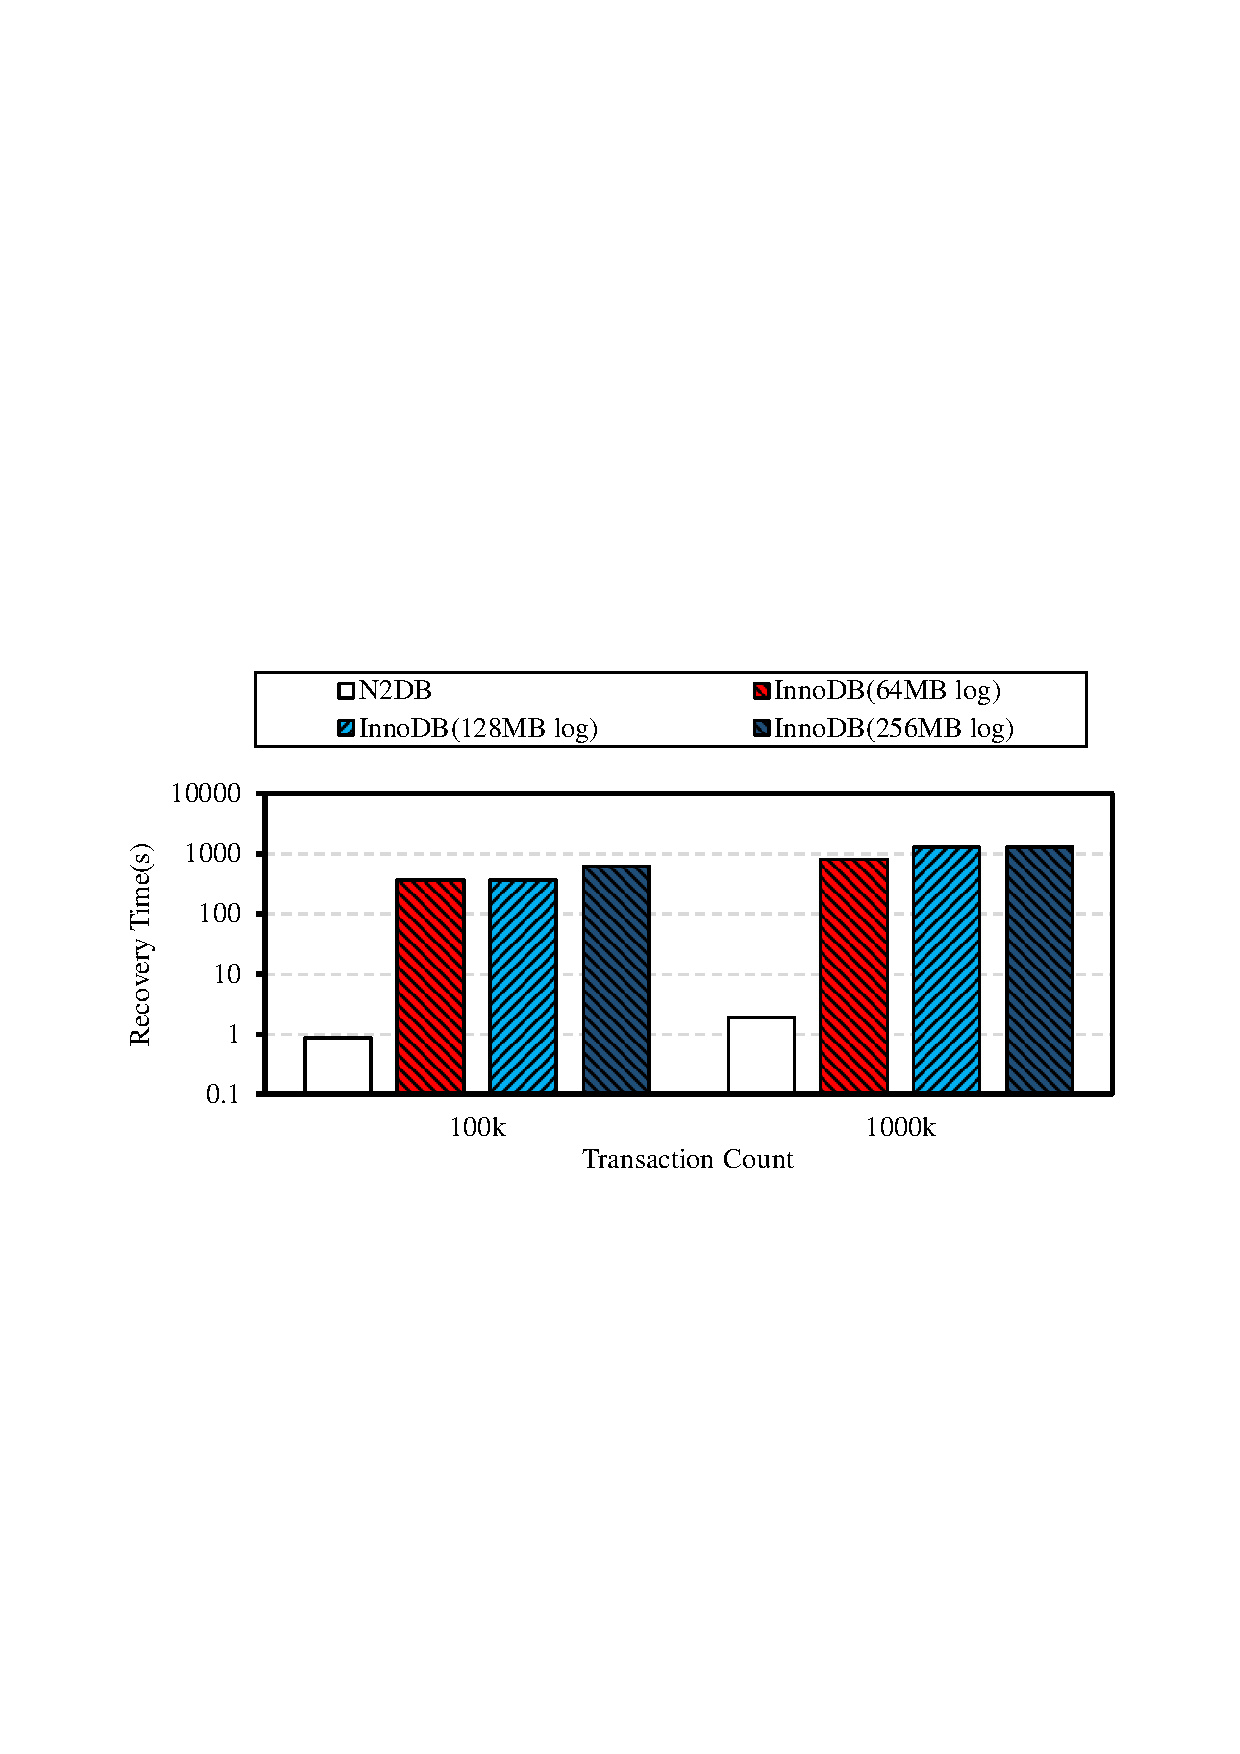
\includegraphics[width=15cm, trim={1cm 9cm 1cm 10cm}]{figures/recovery-time.pdf}
    \caption{YCSB 负载下数据恢复的时间对比实验}
    \label{fig:recovery-time-ycsb}
\end{figure}

\begin{figure}
    \centering
    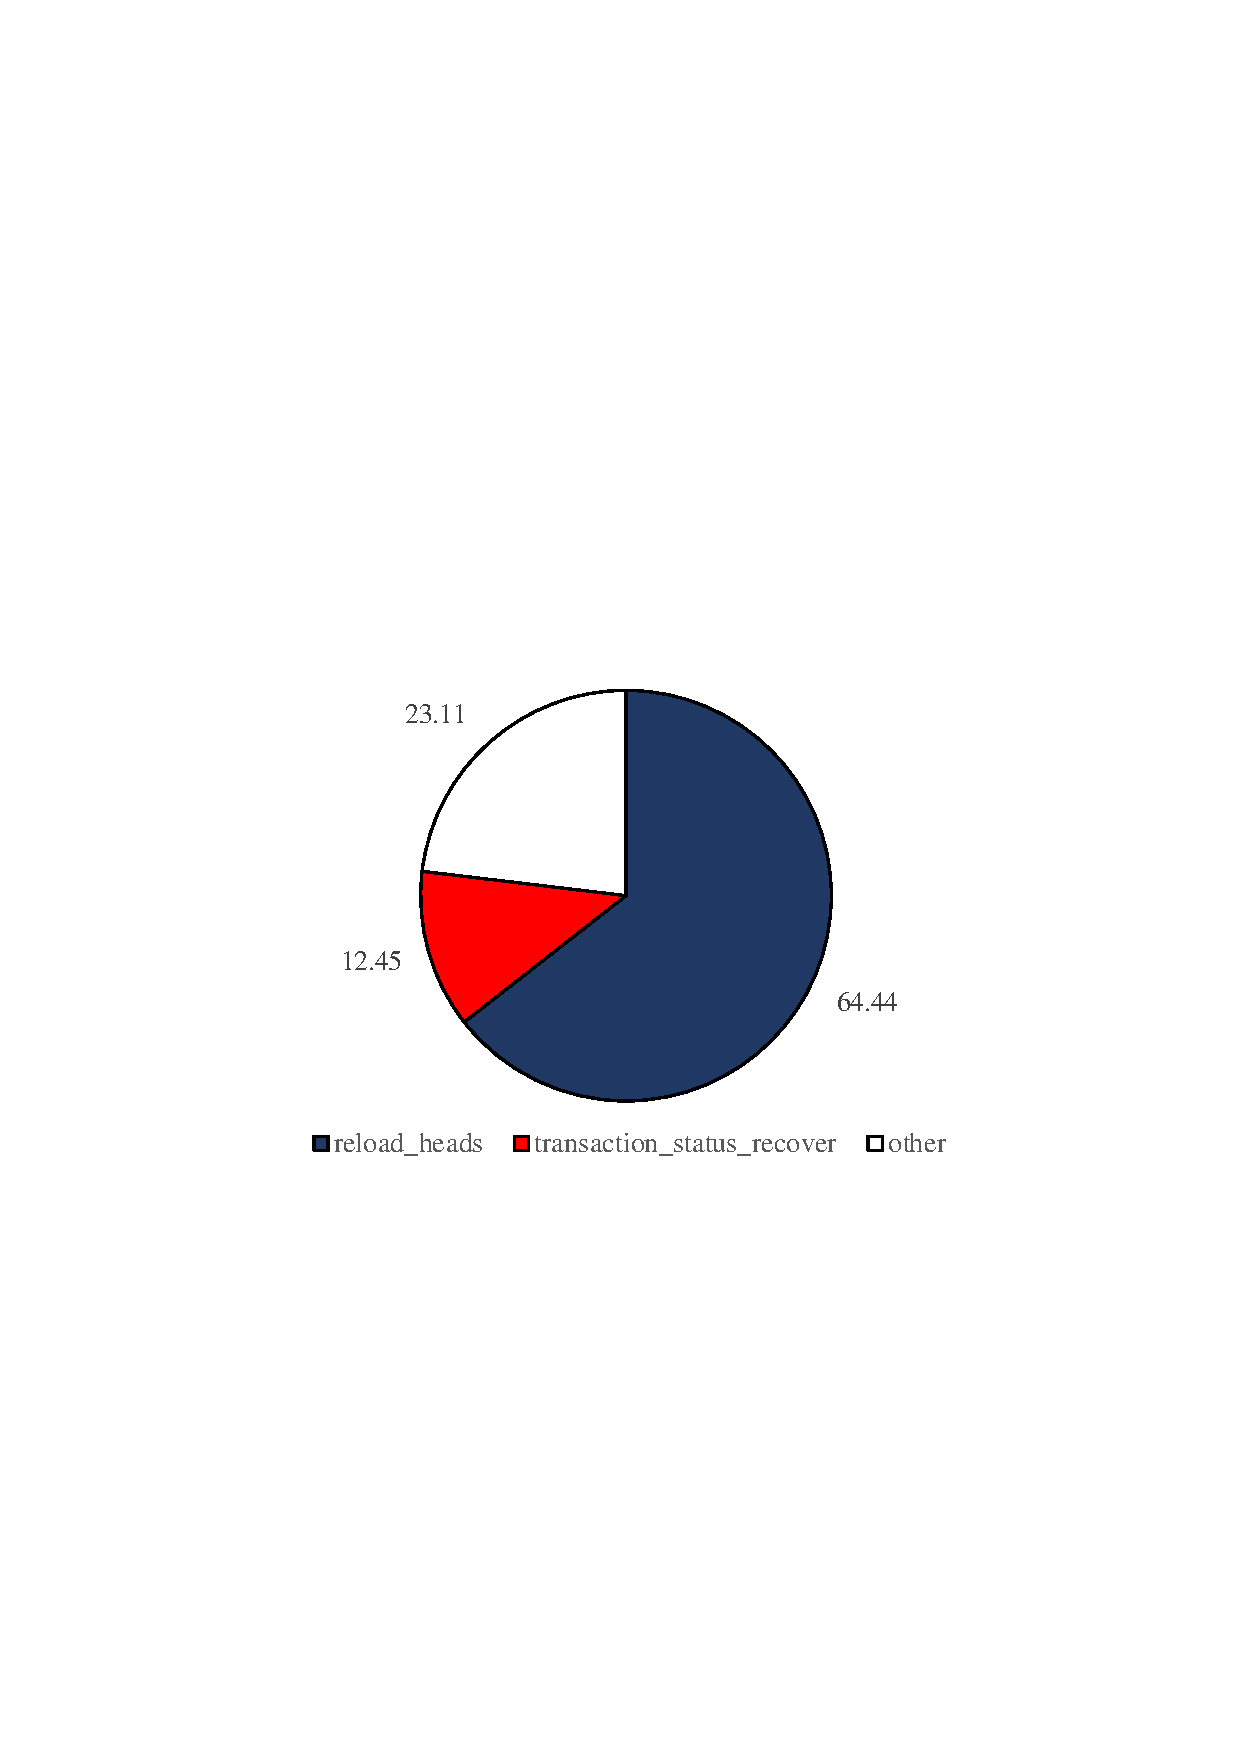
\includegraphics[width=15cm, trim={1cm 9cm 1cm 10cm}]{figures/recovery_perf.pdf}
    \caption{N2DB 的数据恢复性能分析}
    \label{fig:recovery-n2db-perf}
\end{figure}

本章节还分析了两个系统在恢复时的性能分布。
N2DB 的结果展示在图~\ref{fig:recovery-n2db-perf} 中。
从图中可以看出,N2DB 的主要开销在于 reload\_heads。
reload\_heads 的作用是判断所有表格中 head 的可见性。
在目前的实现中,reload\_heads 的开销和表格中 head 的数量成正比。
接下来占比比较大的是事务状态数组的恢复。在数据恢复时系统需要设置之前的事务的状态,将其中未提及的事务的状态设置为 ABORTED。
剩下的元数据恢复以及 NVM 分配器的恢复占了少部分开销。

\begin{figure}
    \centering
    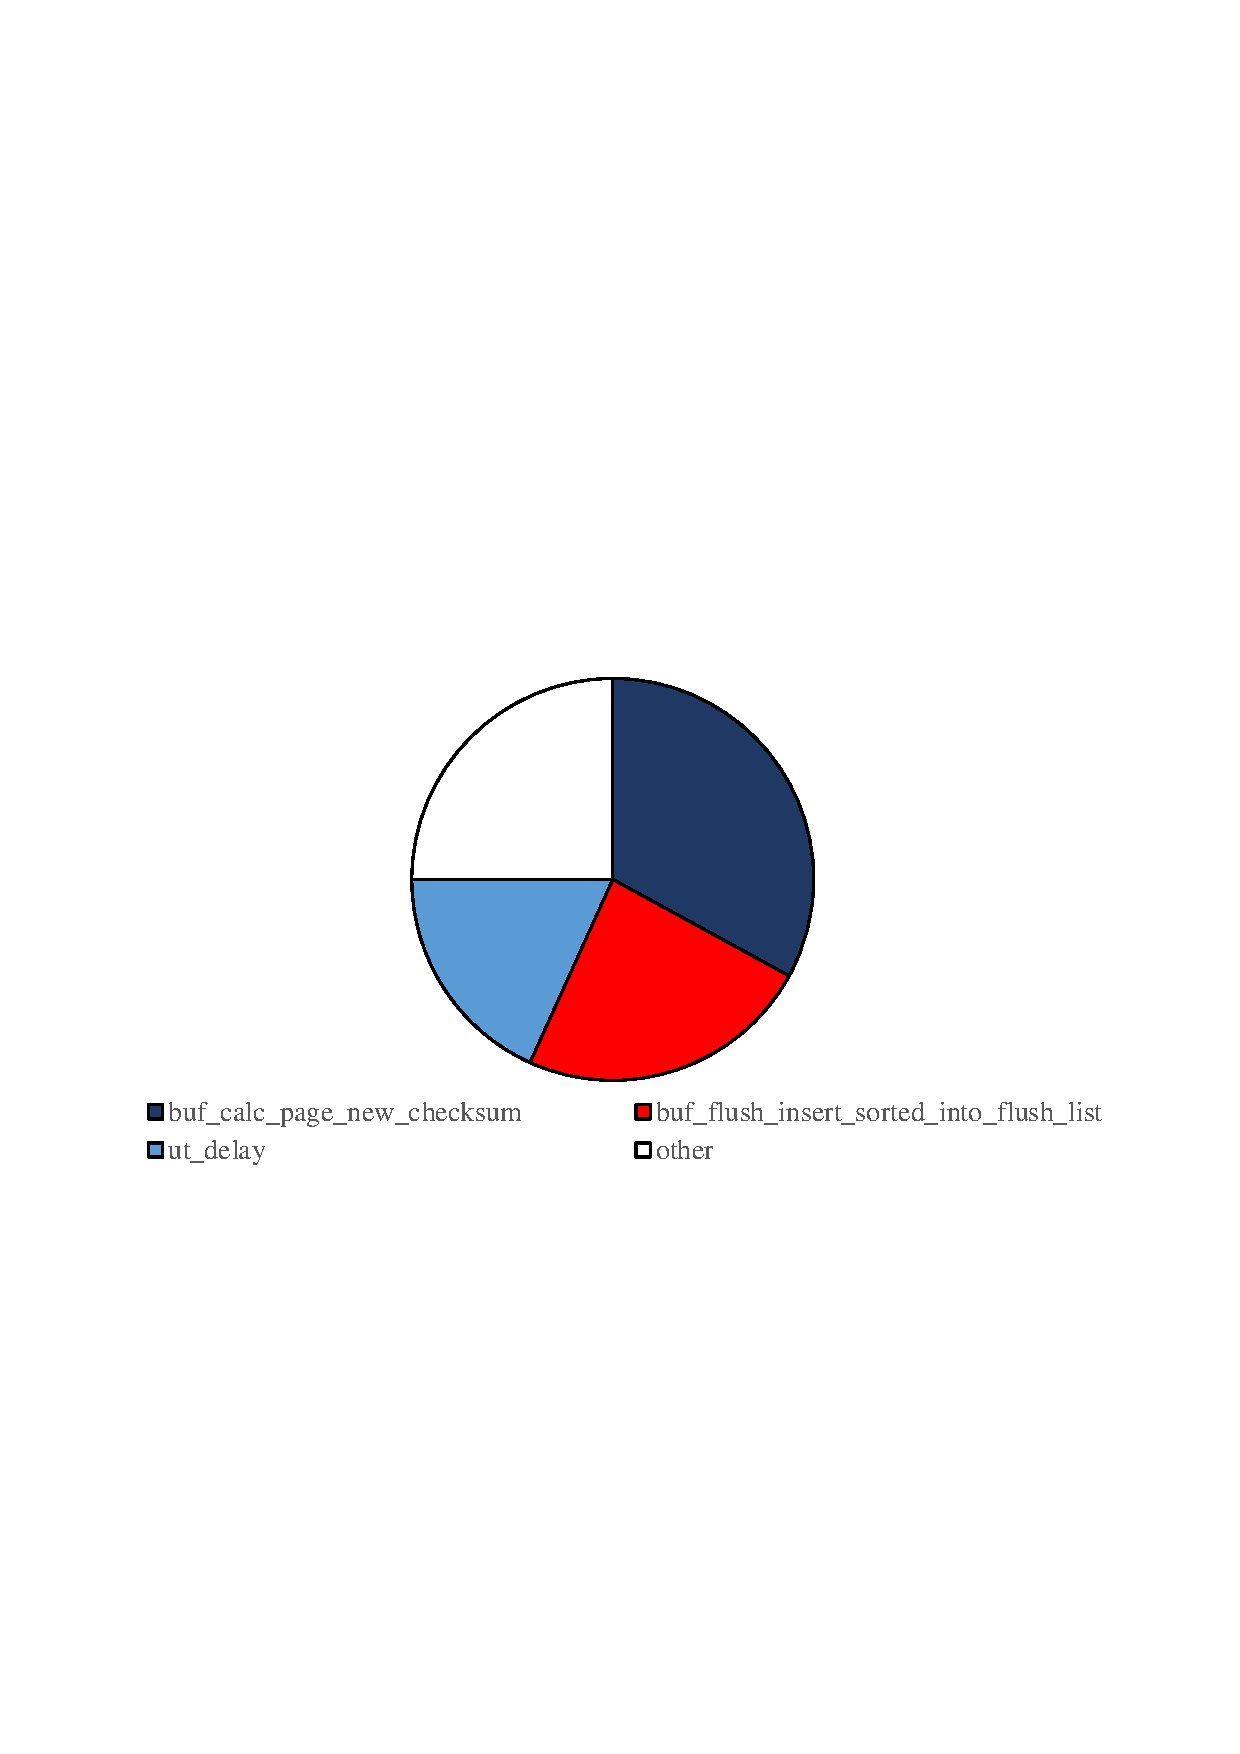
\includegraphics[width=15cm, trim={1cm 9cm 1cm 10cm}]{figures/innodb-recovery-perf.pdf}
    \caption{InnoDB 的数据恢复性能分析}
    \label{fig:recovery-innodb-perf}
\end{figure}


InnoDB 的数据恢复阶段的开销占比如图~\ref{fig:recovery-innodb-perf} 所示。
buf\_flush\_insert\_sorted\_into\_flush\_list 是 InnoDB 在恢复时会调用的数据写回方法。
当 InnoDB 恢复时,其重做阶段和回收阶段都要进行数据的写入。
buf\_calc\_page\_new\_checknum 也是数据写入的一环。
ut\_delay 的开销是由于 InnoDB 在恢复时采用多线程,因此为了避免冲突使用 ut\_delay 来实现自旋锁。

从该开销占比可以看出,InnoDB 在数据恢复阶段的绝大部分开销都是记录数据的修改造成的。
而 N2DB 在数据恢复阶段除了事务状态数组的恢复以外,几乎不需要进行修改操作。
因而 N2DB 的恢复相较于 InnoDB 的 ARIES而言开销极小。








\subsection{存储空间对比}

两个系统的存储空间对比结果展示在图~\ref{fig:recovery-storage-ycsb} 中。
需要注意的是,InnoDB 使用两个日志文件,因此日志的存储空间需要翻倍。
从图中可以看出,N2DB 的存储空间只需要 InnoDB 的一半左右。
主要原因有两点:一是 N2DB 没有日志文件,也不需要存储检查点。
二是相对于 InnoDB 的日志大小,N2DB 的事务状态数组非常轻量。
一百万的事务仅需要 0.2 MB 的存储空间。

\begin{figure}
    \centering
    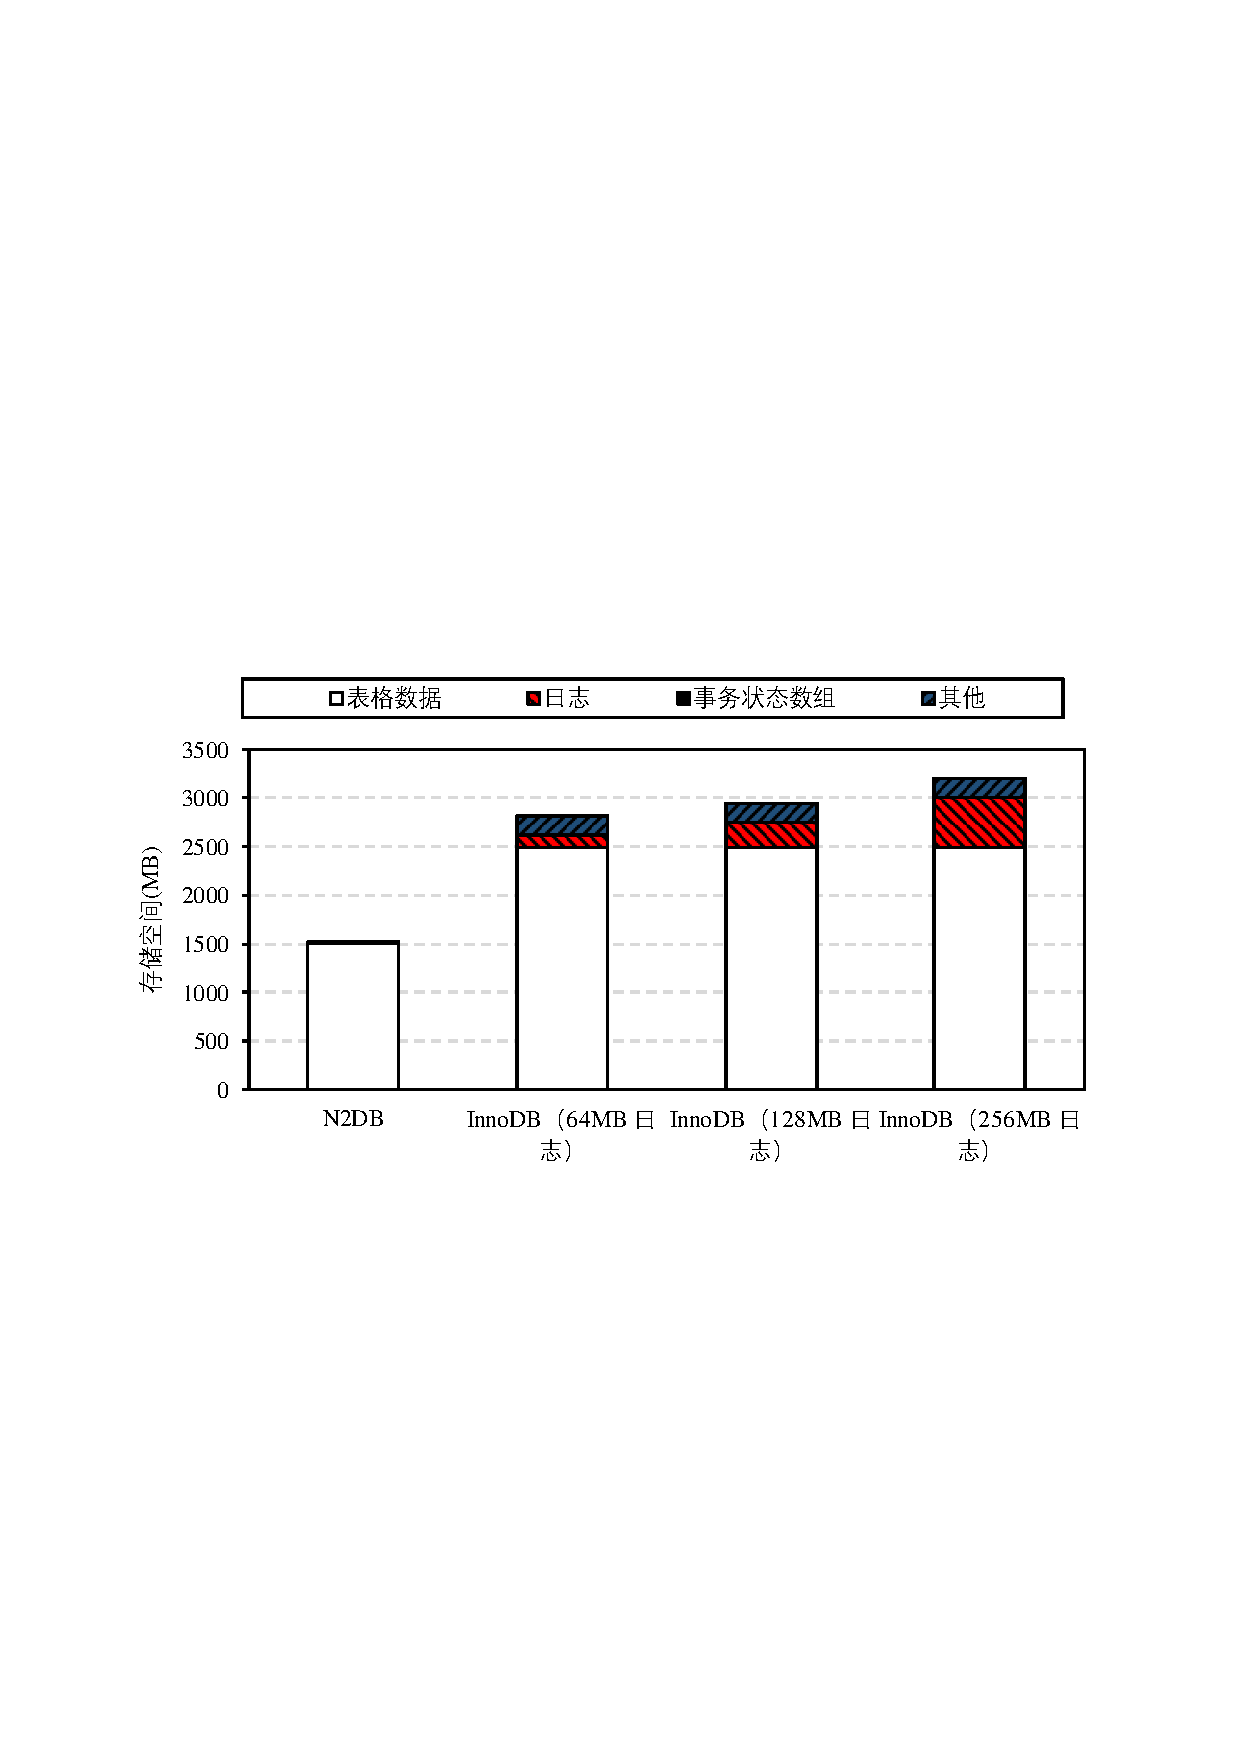
\includegraphics[width=15cm, trim={1cm 9cm 1cm 10cm}]{figures/recovery-storage.pdf}
    \caption{YCSB 负载下垃圾回收性能的存储空间对比实验}
    \label{fig:recovery-storage-ycsb}
\end{figure}



\section{本章小结}

本章节主要对 N2DB 中的垃圾回收机制以及数据恢复机制进行实验,并且对结果进行评估和分析。

首先是垃圾回收机制的性能对比。本章节使用了三种 YCSB 负载以及一种 TPC-C 负载进行测试。相对于关闭垃圾回收的系统,开启垃圾回收的系统在运行时的性能至多降低 $10\%$。但是垃圾回收机制会显著减少存储空间的使用,减少的效果随着事务的更新操作的比例而提升,最高降低 $60\%$ 的存储空间使用。

然后是数据恢复机制的性能对比。实验使用统一的负载以及两种不同的提交事务的阈值。
在两种实验设置中,N2DB 的恢复时间是 InnoDB 的三个数量以下。同时 N2DB 相对于 InnoDB 而言,能够节约 $50\%$ 的存储空间。

综上所述,N2DB 能够在无日志的前提下做到高速地正确地恢复,同时能够有效地利用存储空间,降低对于 NVM 介质的损伤,以保护 NVM 介质的寿命。

